\documentclass{standalone}
\usepackage{tikz}
\begin{document}
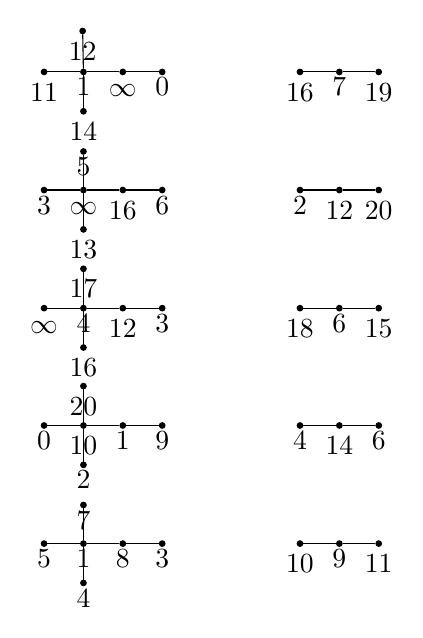
\begin{tikzpicture}[every node/.style={draw, circle, fill=black, minimum size=2pt, inner sep=0pt}]
\node[fill=black, label=below:{\color{black}$11$}] (G1N11) at (4.00,7.00) {};
\node[fill=black, label=below:{\color{black}$1$}] (G1N1) at (4.50,7.00) {};
\node[fill=black, label=below:{\color{black}$\infty$}] (G1Ninf) at (5.00,7.00) {};
\node[fill=black, label=below:{\color{black}$0$}] (G1N0) at (5.50,7.00) {};
\node[fill=black, label=below:{\color{black}$14$}] (G1N14) at (4.50,6.50) {};
\node[fill=black, label=below:{\color{black}$12$}] (G1N12) at (4.49,7.52) {};
\node[fill=black, label=below:{\color{black}$16$}] (G1N16) at (7.25,7.00) {};
\node[fill=black, label=below:{\color{black}$7$}] (G1N7) at (7.75,7.00) {};
\node[fill=black, label=below:{\color{black}$19$}] (G1N19) at (8.25,7.00) {};
\draw (G1N1) -- (G1N11);
\draw (G1N1) -- (G1N14);
\draw (G1N1) -- (G1Ninf);
\draw (G1N1) -- (G1N12);
\draw (G1Ninf) -- (G1N0);
\draw (G1N19) -- (G1N7);
\draw (G1N7) -- (G1N16);
\node[fill=black, label=below:{\color{black}$3$}] (G2N3) at (4.00,5.50) {};
\node[fill=black, label=below:{\color{black}$\infty$}] (G2Ninf) at (4.50,5.50) {};
\node[fill=black, label=below:{\color{black}$16$}] (G2N16) at (5.00,5.50) {};
\node[fill=black, label=below:{\color{black}$6$}] (G2N6) at (5.50,5.50) {};
\node[fill=black, label=below:{\color{black}$13$}] (G2N13) at (4.50,5.00) {};
\node[fill=black, label=below:{\color{black}$5$}] (G2N5) at (4.50,5.99) {};
\node[fill=black, label=below:{\color{black}$2$}] (G2N2) at (7.25,5.50) {};
\node[fill=black, label=below:{\color{black}$12$}] (G2N12) at (7.75,5.50) {};
\node[fill=black, label=below:{\color{black}$20$}] (G2N20) at (8.25,5.50) {};
\draw (G2Ninf) -- (G2N3);
\draw (G2Ninf) -- (G2N13);
\draw (G2Ninf) -- (G2N16);
\draw (G2Ninf) -- (G2N5);
\draw (G2N16) -- (G2N6);
\draw (G2N20) -- (G2N12);
\draw (G2N12) -- (G2N2);
\node[fill=black, label=below:{\color{black}$\infty$}] (G3Ninf) at (4.00,4.00) {};
\node[fill=black, label=below:{\color{black}$4$}] (G3N4) at (4.50,4.00) {};
\node[fill=black, label=below:{\color{black}$12$}] (G3N12) at (5.00,4.00) {};
\node[fill=black, label=below:{\color{black}$3$}] (G3N3) at (5.50,4.00) {};
\node[fill=black, label=below:{\color{black}$16$}] (G3N16) at (4.50,3.50) {};
\node[fill=black, label=below:{\color{black}$17$}] (G3N17) at (4.50,4.50) {};
\node[fill=black, label=below:{\color{black}$18$}] (G3N18) at (7.25,4.00) {};
\node[fill=black, label=below:{\color{black}$6$}] (G3N6) at (7.75,4.00) {};
\node[fill=black, label=below:{\color{black}$15$}] (G3N15) at (8.25,4.00) {};
\draw (G3N4) -- (G3Ninf);
\draw (G3N4) -- (G3N16);
\draw (G3N4) -- (G3N12);
\draw (G3N4) -- (G3N17);
\draw (G3N12) -- (G3N3);
\draw (G3N18) -- (G3N6);
\draw (G3N6) -- (G3N15);
\node[fill=black, label=below:{\color{black}$0$}] (G4N0) at (4.00,2.51) {};
\node[fill=black, label=below:{\color{black}$10$}] (G4N10) at (4.50,2.51) {};
\node[fill=black, label=below:{\color{black}$1$}] (G4N1) at (5.00,2.51) {};
\node[fill=black, label=below:{\color{black}$9$}] (G4N9) at (5.50,2.51) {};
\node[fill=black, label=below:{\color{black}$2$}] (G4N2) at (4.50,2.01) {};
\node[fill=black, label=below:{\color{black}$20$}] (G4N20) at (4.50,3.01) {};
\node[fill=black, label=below:{\color{black}$4$}] (G4N4) at (7.25,2.51) {};
\node[fill=black, label=below:{\color{black}$14$}] (G4N14) at (7.75,2.51) {};
\node[fill=black, label=below:{\color{black}$6$}] (G4N6) at (8.25,2.51) {};
\draw (G4N10) -- (G4N0);
\draw (G4N10) -- (G4N2);
\draw (G4N10) -- (G4N1);
\draw (G4N10) -- (G4N20);
\draw (G4N1) -- (G4N9);
\draw (G4N6) -- (G4N14);
\draw (G4N14) -- (G4N4);
\node[fill=black, label=below:{\color{black}$5$}] (G5N5) at (4.00,1.01) {};
\node[fill=black, label=below:{\color{black}$1$}] (G5N1) at (4.50,1.01) {};
\node[fill=black, label=below:{\color{black}$8$}] (G5N8) at (5.00,1.01) {};
\node[fill=black, label=below:{\color{black}$3$}] (G5N3) at (5.50,1.01) {};
\node[fill=black, label=below:{\color{black}$4$}] (G5N4) at (4.50,0.51) {};
\node[fill=black, label=below:{\color{black}$7$}] (G5N7) at (4.50,1.50) {};
\node[fill=black, label=below:{\color{black}$10$}] (G5N10) at (7.25,1.01) {};
\node[fill=black, label=below:{\color{black}$9$}] (G5N9) at (7.75,1.01) {};
\node[fill=black, label=below:{\color{black}$11$}] (G5N11) at (8.25,1.01) {};
\draw (G5N1) -- (G5N8);
\draw (G5N1) -- (G5N5);
\draw (G5N1) -- (G5N4);
\draw (G5N1) -- (G5N7);
\draw (G5N8) -- (G5N3);
\draw (G5N10) -- (G5N9);
\draw (G5N9) -- (G5N11);
\end{tikzpicture}
\end{document}
